\chapter{SNMP}
\label{kap_snmp}
SNMP, nebo-li Simple Network Management Protocol, je v dnešní době jeden z nejrozšířenějších protokolů na správu počítačové sítě. Je to aplikační protokol, který je součástí TCP/IP rodiny protokolů. 
Byl vyvinut skupinout IETF (Internet Engineering Task Force) a přijat jako standard v roce 1989. Umožňuje sledovat síťový provoz, hledat a řešit problémy, které se při provozu vyskytnou. 

\section{Správní struktura}
SNMP je tvořen sadou standardů, které popisují správu sítě, zahrnující samotný komunikační protokol, definici databázové struktury (SMI) a datové objekty (MIB).

Základním funkčním principem je model Klient - Server (\cite{cisco_snmp}). Struktura spravované sítě se tak dělí na tři klíčové elementy - spravované zařízení, agenta a manažera (viz obrázek \ref{obr_snmp1}).

\begin{figure}[htp]
	\begin{center}
		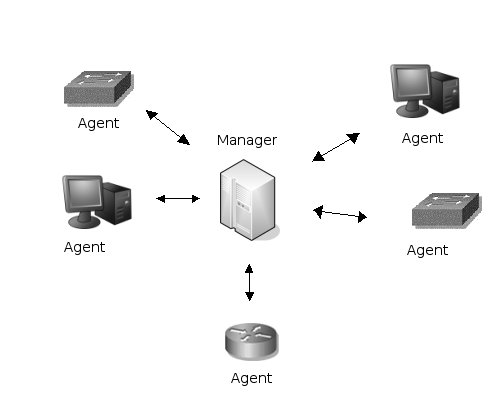
\includegraphics[width=8cm]{obrazky/02_snmp_principle.png}
		\caption{Základní princip fungování SNMP spravované sítě}
		\label{obr_snmp1}
	\end{center}
\end{figure}

\begin{itemize}
	\item \textbf{Spravovaný systém} - je zařízení (přepínač, router, atd.), na kterém je spuštěn SNMP agent. Toto zařízení shromažďuje sledované informace a pak je
	dává k dispozici manažerovi pomocí SNMP protokolu.
	\item \textbf{Agent} - je software určený pro pro správný překlad požadavků manažera a jejích vykonání na sledovaném systému. Navíc může při sledování posílat manažerovi 
	upozornění, že něco není se systémem v pořádku.
	\item \textbf{Manažer} (NMS - Network Managemet System) - je aplikace, která sleduje a spravuje všechny systémy na sledované síti. Tento systém získává od agentů data, zpracovává je do vizuální podoby, 
	čímž dává možnost administrátorovi mít přehled o celé síti. Zároveň umožňuje měnit sledované parametry přímo u agenta.
\end{itemize}

Komunikace můžeme rozdělit do dvou kategorií dle toho, kdo jí započal. Základní schéma je vyjádřeno na obrázku \ref{obr_snmp2} (\cite{tcpip_snmp}).

\begin{figure}[htp]
	\begin{center}
		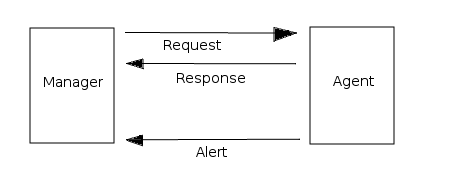
\includegraphics[width=12cm]{obrazky/02_snmp_communication.png}
		\caption{Komunikace mezi SNMP manažerem a agentem}
		\label{obr_snmp2}
	\end{center}
\end{figure}

V první části schématu je vyobrazeno standardní chování managera, který posílá dotazy agentovi, který mu odpovídá. Přesný výpis příkazů a zpráv, které si mohou tyto dva systémy mezi sebou vyměňovat, bude 
diskutován dále v této kapitole.

Druhá část schématu popisuje moment, kdy na sledovaném systému nastala nějaká extrémní situace (např. zatížení síťového spoje se blíží k maximu) a agent informuje manažera pomocí zprávi Alert (v SNMP jsou to zprávy
TRAP či INFORM, obě budoudiskutovány dále).

Je nutné zmínit, že SNMP protokol pracuje nad transportním protokolem UDP, který je nepotvrzovaný. Není tedy zaručeno, že bude komunikace probíhat bezchybně. Je možné, že některé dotazy a příkazy vůbec nedojdou
ke svému cíli, o čemž se druhá strana nikdy nedozví. Tento fakt může být překážkou při správě rozsáhlých sítí, kde jsou špatné síťové spoje.


\section{SMI, MIB standardy}
Jak již bylo zmíněno dříve, SNMP je sada standardů, která kromě komunikačního protokolu musí definovat i strukturu sledované databáze a samotná data. Tyto informace byly definovány ve standardech SMI a MIB.

\subsection*{SMI}
SMI je zkratkou pro Structure and Identification of Management Information for TCP/IP-based Internets. Tento standard (\cite{rfc1155}) popisuje a definuje základní datové struktury a typy, které protokol využívá.
Jednotlivé objekty jsou pojmenovány a organizovány, aby bylo možné k těmto datům logicky přistupovat. Dle standardu musí mít každý objekt jméno, syntaxi a kódování. Jméno jednoznačně identifikuje objekt. Datový typ
(číslo, řetězec) je určen syntaxí. Kódování zajišťuje správnou serializaci dat při přenosu mezi systémy.

Objekty, identifikovány svým jménem (OID), jsou seřazeny do hierarchické struktury. K identifikaci je použito Abstract Syntax Notation One (ASN.1). Každý OID identifikátor je složen ze skupiny přirozených čísel, které
vyjadřují jeho pozici v pomyslném stromu. Strom má kořen, který je spojen hranami s očíslovanými uzly. Každý uzel může mít vlastní děti, čímž tvoří vlastní podstrom. Takto je možno pokračovat dále do značné hloubky stromu. 
Tento standard též specifikuje, jaké identifikátory jsou přiřazeny počátku správní databáze.

\subsection*{MIB}
MIB je zkratka pro Management Information Base. Je to soubor definicí, které popisují parametry a vlastnosti sledovaného zařízení. Existuje více než 100 různých MIB, které popisují různá zařízení. Každý takovýto
soubor definic musí splňovat předpisy SMI, aby bylo zaručena správná interpretace objektů. Každý objekt (někdy také nazýván MIB objekt) je unikátně identifikován svým OID a všechny dohromady jsou uspořádány do
stromové struktury tak, jak to bylo popsáno v minulém odstavci. 

Objekty v dané databázi se dělí na \textit{skalární} a \textit{tabelární}. Skalární objekty reprezentují jeden parametr sledovaného zařízení (např. počet ethernetových karet v přepínači), kdežto tabelární objekty
jsou spojením několika spřízněných objektů (např. routovací tabulka je spojením jednotlivých záznamů, coby řádků dané tabulky).

V rámci hierarchického uspořádání jsou vyhrazeny vyšší úrovně stromu (blíže kořenu) jednotlivým standardizujícím organizacím, nižší úrovně jsou poté zadány jednotlivými společnostmi. Každý výrobce si může definovat svojí
privátní větev, do které umístí specifické informace daného zařízení.

MIB, které nebyly standardizovány a oficiálně schváleny, jsou umístěny do větve experimentální.


\section{Verze SNMP protokolu}
Celkem byly doposud standardizovány tři verze protokolu SNMP. Každá z nich definuje svoje specifické datové typy a používané datové rámce pro komunikaci. 

\subsection*{SNMPv1}
V první verzi protokolu byly definovány dvě skupiny datových typů:
\begin{itemize}
	\item Základní datové typy (Simple data types)
	\item Aplikační typy
\end{itemize}

Základní typy jsou definovány v SNMPv1 SMI a definují základní používané hodnoty:
\begin{itemize}
	\item \textbf{INTEGER} - celá čísla od $ -2^{31} $ do $ 2^{31}-1$
	\item \textbf{OCTET STRING}
	\item \textbf{OBJECT IDENTIFIER} - identifikace jednotlivých objektů v rámci normy ASN.1
\end{itemize}

Aplikační specifické typy pak jsou:
\begin{itemize}
	\item \textbf{Network Address} - obecná síťová adresa pro podporu mnoha rodin protokolů.
	\item \textbf{IpAddress} - přímo definovaný typ pro IP adresu. SMIv1 podporuje pouze 32 bitovou adresu (IPv4)
	\item \textbf{Counter} - čítač, vyjádřen celým číslem bez znaménka; Jeho hodnota se pouze zvyšuje a to až do maxima a pak se vrací zpět na nulu
	\item \textbf{Gauge} - je definována jako nezáporné celé číslo. Může hodnotu zvyšovat i snižovat a to v definovaných mezích minima a maxima
	\item \textbf{Time Ticks} - počet hodinových tiků od nějaké události, měřeno v setinách vteřiny
	\item \textbf{Opaque} - typ dovolující přenášet libovolná data v kódování ASN.1. Tato data jsou zakódována jako OCTET STRING a následně přenesena médiem.
	\item \textbf{Integers} - celočíselný typ, který předefinovává specifikaci v SMI
	\item \textbf{Unsigned Integer} - celočíselný typ bez znaménka, který stejně jako předchozí předefinovává specifikaci.
\end{itemize}

Komunikační mechanismus mezi manažerem a agentem je definován pomocí datových rámců, které je možné v rámci SNMPv1 přenášet. Tyto jsou:
\begin{itemize}
	\item \textbf{Get Request} - získání hodnoty uzlu identifikovaného OID (zpráva od manažera agentovi)
	\item \textbf{Get Next Request} - žádost o hodnotu uzlu následujícího po zaslaném OID (od manažera k agentovi)
	\item \textbf{Set Request} - Nastavení hodnoty uzlu specifikovaném OID (od manažera k agentovi) 
	\item \textbf{Get Response} - odpověď agenta manažerovi na Get a Set zprávy. Obsahují požadovanou hodnotu
	\item \textbf{Trap} - zpráva od agenta manažerovi, která upozorňuje na nastálé situace na monitorovaném systému.
\end{itemize}

Strukturu jednotlivých SNMP paketů zobrazuje obrázek \ref{obr_snmp3}.

\begin{figure}[htp]
	\begin{center}
		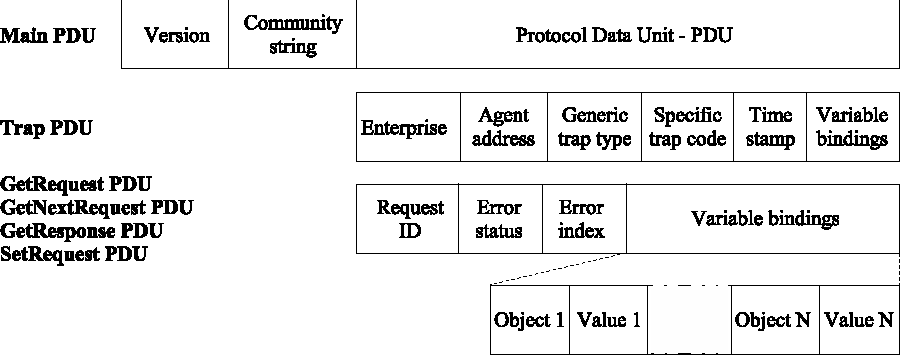
\includegraphics{obrazky/02_snmp_pdu.pdf}
		\caption{Schéma datových paketů protokolu SNMPv1 a v2 (\cite{macejko_dipl})}
		\label{obr_snmp3}
	\end{center}
\end{figure}

Hlavní část datového paketu je tvořena poli Version a Community string. První popisuje verzi SNMP protokolu použitou při komunikaci a druhé je heslo pro přístup
k položkám MIB. Blíže k bezpečnosti v dalším odstavci. Druhá část paketu se liší dle typu zprávy. Paket odeslaný agentem při výskytu monitorované události obsahuje
informace, které popisují druh problému.
\begin{itemize}
	\item \textit{Enterprise} - identifikuje typ zařízení, které zprávu poslalo
	\item \textit{Agent adress} - adresa zařízení, kde běží agent
	\item \textit{Generic trap type} - specifikuje, zda-li se jednalo o některý z předdefinovaných typů událostí (linkDown, linkUp, coldStart, aj.)
	\item \textit{Specific trap type} - identifikuje jednu z mnoha specifických událostí
\end{itemize}

Druhým typem zprávy jsou dotazy a odpovědi, které zasílá manažer a agent na ně odpovídá. Jednotlivá pole mají následující význam:
\begin{itemize}
	\item \textit{Request ID} - pořadové číslo dotazu (aby manažer věděl, na co přišla odpověď)
	\item \textit{Error status} - je nastaven pouze u odpovědi a obsahuje druh problému, který se při dotazu objevil
	\item \textit{Error index} - asociuje problém s instancí objektu.
\end{itemize}

Společným polem pro oba dva typy paketu jsou \textit{Variable bindings} - jsou to dvojice polí, kde jedna část identifikuje objekt a druhá část je jeho hodnota. Například
při dotazu příkazem GET se nastaví název objektu a v odpovědi přijde nastavena i hodnota.

Bezpečnost v této verzi protokolu je založena pouze na takzvaném \textit{community string}u, který vystupuje jako heslo. Existují pouze dvě úrovně zabezpečení
přístupu a to - pouze pro čtení (read only) a čtení-zápis (read-write access). Je patrné, že se používají pouze dvě hesla, každé pro jednu úroveň. Je to velice slabé
zabezpečení, vezmeme-li v úvahu, že toto heslo se posílá nezašifrované a každý, kdo dokáže odchytit jednotlivé pakety, si může tento řetězec přečíst. Tento nedostatek
se pokoušejí odstranit až další verze protokolu.

\subsection*{SNMPv2}
Druhá verze protokolu SNMP byla zaměřena na odstranění nedostatků verze první. Bohužel bylo vydáno několik soupeřících specifikací, označované názvy SNMPv2c, SNMPv2u, SNMPv2*, které
byly vzájemně nekompatibilní. Nicméně zlepšení oproti první verzi bylo několik. Byly definovány nové datové typy, nové zprávy a zlepšená práce s chybami.

Nové datové typy zahrnují rozšíření podpory z 32-bitových čísel na 64-bitová ( Integer32, Integer64, Counter32, ...). 

Přidané zprávy jsou:
\begin{itemize}
	\item \textbf{Get Bulk} - tento operátor se snaží efektivněji využít přenosovou kapacitu kanálu tím, že od agenta si vyžádá sérii informací pomocí jediného dotazu.
	\item \textbf{Inform} - stejná funkcionalita jako zpráva Trap ve verzi 1, ale nutné je potvrzení od manažera, že zprávu přijal (Response paket)
	\item \textbf{Response} - odpověď na předcházející Inform zprávu (od manažera k agentovi)
\end{itemize}

Ostatní zprávy SNMPv2 přebírá z předchozí verze a zachovává jejich strukturu. Stejně tak je to i s bezpečností, kde je stále použito heslo ve smyslu community stringu.

\subsection*{SNMPv3}
Třetí verze protokolu SNMP je definována sadou standardů, které nepostihují celkovou funkčnost protokolu jako takového, ale 
dodávají do systému chybějící prvky, hlavně bezpečnosti. Přímo v jednom ze standardů \cite{rfc2570} je řečeno, že tato verze může být chápána jako 
SNMPv2 s dodatečnými administrativními a bezpečnostními schopnostmi.

SNMPv3 definuje tři základní služby:
\begin{itemize}
	\item \textit{Autentifikaci} - datový přenos od manažera k agentovi může být autentifikován, aby se zajistilo ověření identity odesílajícího.
	\item \textit{Soukromí} - šifrování přenášených zpráv.
	\item \textit{Přístupová práva} - agent může definovat přístupová práva, omezovat přístup manažerům k pouze některým akcím a částem dat.
\end{itemize}

Základním principem SNMPv3 je modularita. Každá SNMP entita je tvořena SNMP řídícím systémem a vlastní aplikací. Řídící systém má za úkol 
přijímat, odesílat, šifrovat, dešifrovat všechny zprávy a dále spravuje a kontroluje monitorované objekty. Tyto funkce jsou poté k dispozici jedné či více
aplikací.

Stejně jako předchozí verze, je SNMPv3 založena primárně na transportním protokolu UDP, ale není na něj vázána. Pro přenos dat tak může být použit i jiný protokol.
Vlastní aplikační protokol SNMP je rozdělen do dvou úrovní. První zpracovává datové pakety (PDU processing layer) a druhá zpracovává zprávy (message processing layer).
Nejvyšší úroveň - PDU processing layer - se stará o zpracování příkazů (Get, Get Next, ...), které přijdou v daném paketu. Zpracovaný paket pak předá nižší úrovni - 
message processing layer - která tomuto paketu dodá hlavičku, kde jsou uložena bezpečnostní data.

Na obrázku \ref{obr_snmp4} je vyobrazen formát SNMPv3 zprávy. První část je tvořena systémem zpracování zpráv. Nese informace ohledně verzi protokolu, identifikaci zprávy,
maximální délce zprávy a nastavení bezpečnostího modelu. Druhá část je generována bezpečnostním systémem a obsahuje informace o kódování a autorizaci. Třetí část obsahuje samotná 
data.

\begin{figure}[htp]
	\begin{center}
		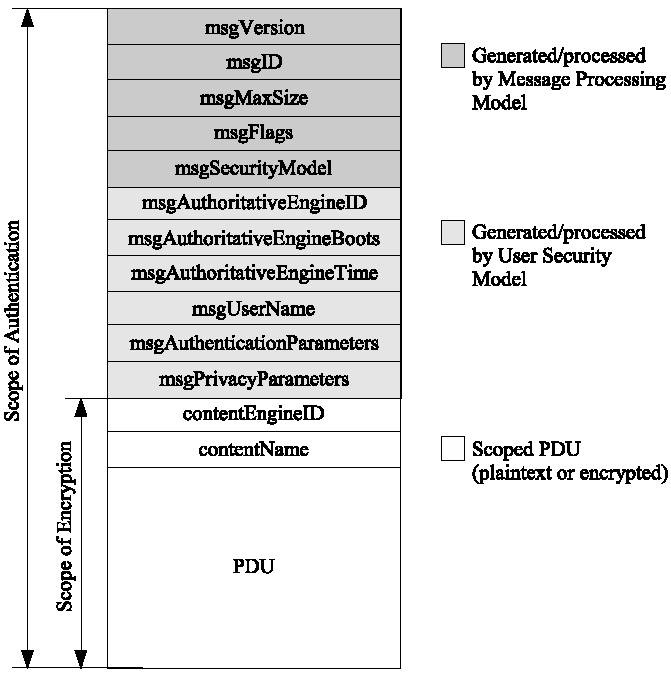
\includegraphics{obrazky/02_snmpv3_pdu.pdf}
		\caption{Schéma datového paketu protokolu SNMPv3 (\cite{macejko_dipl})}
		\label{obr_snmp4}
	\end{center}
\end{figure}


Důležitou součástí nového standardu je i systém přístupových práv (VACM - View-Based Access Control Model). Tento model umožňuje nakonfigurovat agenta tak, 
že specifickému manažerovi bude umožněn přístup pouze k části MIB. Je možné omezit manažera pro přístup pouze k části databáze monitorovaných dat a 
zároveň ještě omezit operace, které nad touto množinou může provádět. Omezení přístupu se provádí pro definované skupiny, kde součástí jedné skupiny může být
více manažerů.

